\documentclass[a4paper, 12pt]{article}
\usepackage[a4paper,top=1.5cm, bottom=1.5cm, left=1cm, right=1cm]{geometry}
\usepackage[utf8]{inputenc}
\usepackage{mathtext}
\usepackage{amsmath}
\usepackage{amsfonts}
\usepackage[english, russian]{babel}
\usepackage{indentfirst}
\usepackage{longtable}
\usepackage{graphicx}
\graphicspath{{pictures/}}
\DeclareGraphicsExtensions{.pdf,.png,.jpg}
\usepackage{natbib}
\usepackage{hyperref}

\title{Лабораторная работа 1.1.3. Статистическая обработка результатов многократных измерений}
\author{Платонов Егор}
\date{\today}



\begin{document}
	
\maketitle


\section{Аннотация}
\textbf{Цель}: применение методов обработки экспериментальных данных при измерении сопротивлений.

\textbf{В работе используется}: набор резисторов (270 штук), цифровой вольтметр, использующийся в режиме омметра.

\section{Теоретические сведения}
В массовом производстве резисторов есть много факторов, влияющих на точность изготовления и избежать отклонений от номинала невозможно. Плохая настройка аппаратуры и станков приводит к систематическим погрешностям, а неоднородные химический состав и толщина проволоки, например, могут привести к случайным погрешностям.

Погрешностью измерительного прибора можно пренебречь, так как она незначительна по сравнению с отклонениями от номинала, в силу точности прибора.


\section{Результаты измерений и обработка данных}

В таблице 1 приведены результаты измерения сопротивлений 270 резисторов (в порядке возрастания). По этим данным построена гистограмма (на рисунке 1 число разбиений $m=$ 10, на рисунке 2 число разбиений $m=$ 20). Чтобы гистограмму можно было сравнить с нормальным распределением, на оси оридинат отложено не число результатов, попадающих в интервал ($\Delta n$), а $\omega = \frac{\Delta n}{N\Delta R}$, где $N$ -- число всех результатов, а $\Delta R$ -- величина интервала измерения.

В таблицах 2 и 3 в зависимости от номера интервала $k$ приведены значения $\Delta n$ и $\omega$.

Вычислим среднее значение сопротивления резисторов:

\begin{equation}
    \overline{R}=\frac{1}{N}\sum_{i=1}^N R_i = 499,56 \text{ Ом}
\end{equation}

И среднеквардатическое отклонение:

\begin{equation}
    \sigma=\sqrt{\frac{1}{N}\sum_{i=1}^N(R_i-\overline{R})^2} \approx 1,34\text{ Ом}
\end{equation}

В интервал $[\overline{R}-\sigma; \overline{R}+\sigma]$ попадает 72,6\% результатов, в интервал $[\overline{R}-2\sigma; \overline{R}+2\sigma]$ 94,8\% результатов, в интервал $[\overline{R}-3\sigma; \overline{R}+3\sigma]$ 98,5\% результатов, в интервал $[\overline{R}-4\sigma; \overline{R}+4\sigma]$ 99,6\% результатов, в интервал $[\overline{R}-5\sigma; \overline{R}+5\sigma]$ 100\% результатов. Точки на оси абсцисс $(\overline{R} \pm \sigma)$, $(\overline{R} \pm 2\sigma)$, $(\overline{R} \pm 3\sigma)$, $(\overline{R} \pm 4\sigma)$, $(\overline{R} \pm 5\sigma)$ отмечены на рисунках 1 и 2 синими линиями.

Для посторения графика нормального распределения используется формула:

\begin{equation}
    y(R)=\frac{1}{\sigma\sqrt{2\pi}}e^{-\frac{(R-\overline{R})^2}{2\sigma^2}}
\end{equation}

Эта зависимость изображена на риунках 1 и 2 красной линией.

\begin{table}[!ht]
    \label{tab:table}
    \caption{Результаты измерения сопротивлений 270 резисторов}
    \centering
    \begin{tabular}{|l|l|l|l|l|l|l|l|l|l|}
    \hline
        494,3 & 494,3 & 496,6 & 496,8 & 497 & 497,2 & 497,3 & 497,6 & 497,6 & 497,6 \\ \hline
        497,6 & 497,6 & 497,8 & 497,8 & 497,9 & 497,9 & 498 & 498 & 498 & 498 \\ \hline
        498 & 498 & 498 & 498 & 498 & 498 & 498 & 498 & 498,1 & 498,1 \\ \hline
        498,1 & 498,1 & 498,1 & 498,2 & 498,2 & 498,2 & 498,2 & 498,3 & 498,3 & 498,3 \\ \hline
        498,3 & 498,3 & 498,3 & 498,4 & 498,4 & 498,4 & 498,4 & 498,5 & 498,5 & 498,5 \\ \hline
        498,5 & 498,5 & 498,5 & 498,6 & 498,6 & 498,6 & 498,6 & 498,6 & 498,6 & 498,7 \\ \hline
        498,7 & 498,7 & 498,7 & 498,7 & 498,7 & 498,7 & 498,8 & 498,8 & 498,8 & 498,8 \\ \hline
        498,8 & 498,8 & 498,8 & 498,8 & 498,8 & 498,8 & 498,9 & 498,9 & 498,9 & 498,9 \\ \hline
        498,9 & 498,9 & 499 & 499 & 499 & 499 & 499 & 499 & 499 & 499 \\ \hline
        499,1 & 499,1 & 499,1 & 499,1 & 499,1 & 499,1 & 499,1 & 499,1 & 499,1 & 499,1 \\ \hline
        499,1 & 499,1 & 499,1 & 499,1 & 499,1 & 499,1 & 499,1 & 499,2 & 499,2 & 499,2 \\ \hline
        499,2 & 499,2 & 499,2 & 499,2 & 499,2 & 499,3 & 499,3 & 499,3 & 499,3 & 499,3 \\ \hline
        499,3 & 499,3 & 499,3 & 499,3 & 499,3 & 499,4 & 499,4 & 499,4 & 499,4 & 499,4 \\ \hline
        499,4 & 499,4 & 499,4 & 499,4 & 499,4 & 499,5 & 499,5 & 499,5 & 499,5 & 499,5 \\ \hline
        499,5 & 499,5 & 499,5 & 499,5 & 499,5 & 499,5 & 499,5 & 499,6 & 499,6 & 499,6 \\ \hline
        499,6 & 499,6 & 499,6 & 499,6 & 499,6 & 499,6 & 499,6 & 499,7 & 499,7 & 499,7 \\ \hline
        499,7 & 499,7 & 499,8 & 499,8 & 499,8 & 499,8 & 499,8 & 499,8 & 499,8 & 499,8 \\ \hline
        499,8 & 499,8 & 499,8 & 499,9 & 499,9 & 499,9 & 499,9 & 499,9 & 499,9 & 500 \\ \hline
        500 & 500 & 500 & 500 & 500 & 500 & 500 & 500,1 & 500,1 & 500,1 \\ \hline
        500,1 & 500,1 & 500,1 & 500,1 & 500,1 & 500,1 & 500,1 & 500,1 & 500,2 & 500,2 \\ \hline
        500,2 & 500,2 & 500,3 & 500,3 & 500,3 & 500,3 & 500,3 & 500,4 & 500,4 & 500,4 \\ \hline
        500,4 & 500,4 & 500,4 & 500,4 & 500,5 & 500,5 & 500,5 & 500,5 & 500,6 & 500,7 \\ \hline
        500,7 & 500,7 & 500,7 & 500,8 & 500,8 & 500,8 & 500,8 & 500,8 & 500,8 & 500,8 \\ \hline
        500,9 & 500,9 & 500,9 & 501 & 501 & 501 & 501 & 501,1 & 501,1 & 501,2 \\ \hline
        501,2 & 501,2 & 501,2 & 501,3 & 501,3 & 501,3 & 501,4 & 501,4 & 501,4 & 501,5 \\ \hline
        501,6 & 501,6 & 501,6 & 501,6 & 501,8 & 501,9 & 502 & 502,2 & 502,2 & 502,2 \\ \hline
        502,4 & 502,4 & 502,4 & 502,5 & 502,6 & 502,6 & 502,8 & 502,8 & 503,7 & 505,5 \\ \hline
    \end{tabular}
\end{table}

\begin{table}[!ht]
    \caption{}
    \centering
    \begin{tabular}{|l|l|l|l|l|l|l|l|l|l|l|}
    \hline
        $k$ & 1 & 2 & 3 & 4 & 5 & 6 & 7 & 8 & 9 & 10 \\ \hline
        $\Delta n$ & 2 & 0 & 10 & 54 & 113 & 58 & 20 & 11 & 1 & 1 \\ \hline
        $\omega, 10^{-3}$ & 7 & 0 & 33 & 179 & 374 & 192 & 66 & 36 & 3 & 3 \\ \hline
    \end{tabular}
\end{table}

\begin{table}[!ht]
    \caption{}
    \centering
    \begin{tabular}{|l|l|l|l|l|l|l|l|l|l|l|}
    \hline
        $k$ & 1 & 2 & 3 & 4 & 5 & 6 & 7 & 8 & 9 & 10 \\ \hline
        $\Delta n$ & 2 & 0 & 0 & 0 & 3 & 7 & 25 & 29 & 59 & 54 \\ \hline
        $\omega, 10^{-3}$ & 13 & 0 & 0 & 0 & 20 & 46 & 165 & 192 & 390 & 357 \\ \hline
    \end{tabular}
\end{table}
\begin{table}[!ht]
    \centering
    \begin{tabular}{|l|l|l|l|l|l|l|l|l|l|l|}
    \hline
        $k$ & 11 & 12 & 13 & 14 & 15 & 16 & 17 & 18 & 19 & 20 \\ \hline
        $\Delta n$ & 35 & 23 & 13 & 7 & 9 & 2 & 1 & 0 & 0 & 1 \\ \hline
        $\omega, 10^{-3}$ & 231 & 152 & 86 & 46 & 60 & 13 & 7 & 0 & 0 & 7 \\ \hline
    \end{tabular}
\end{table} 

\begin{figure}[h!]
\centering
\label{hist1}
\caption{Гисторамма ($m=$10) и нормальное распределение}
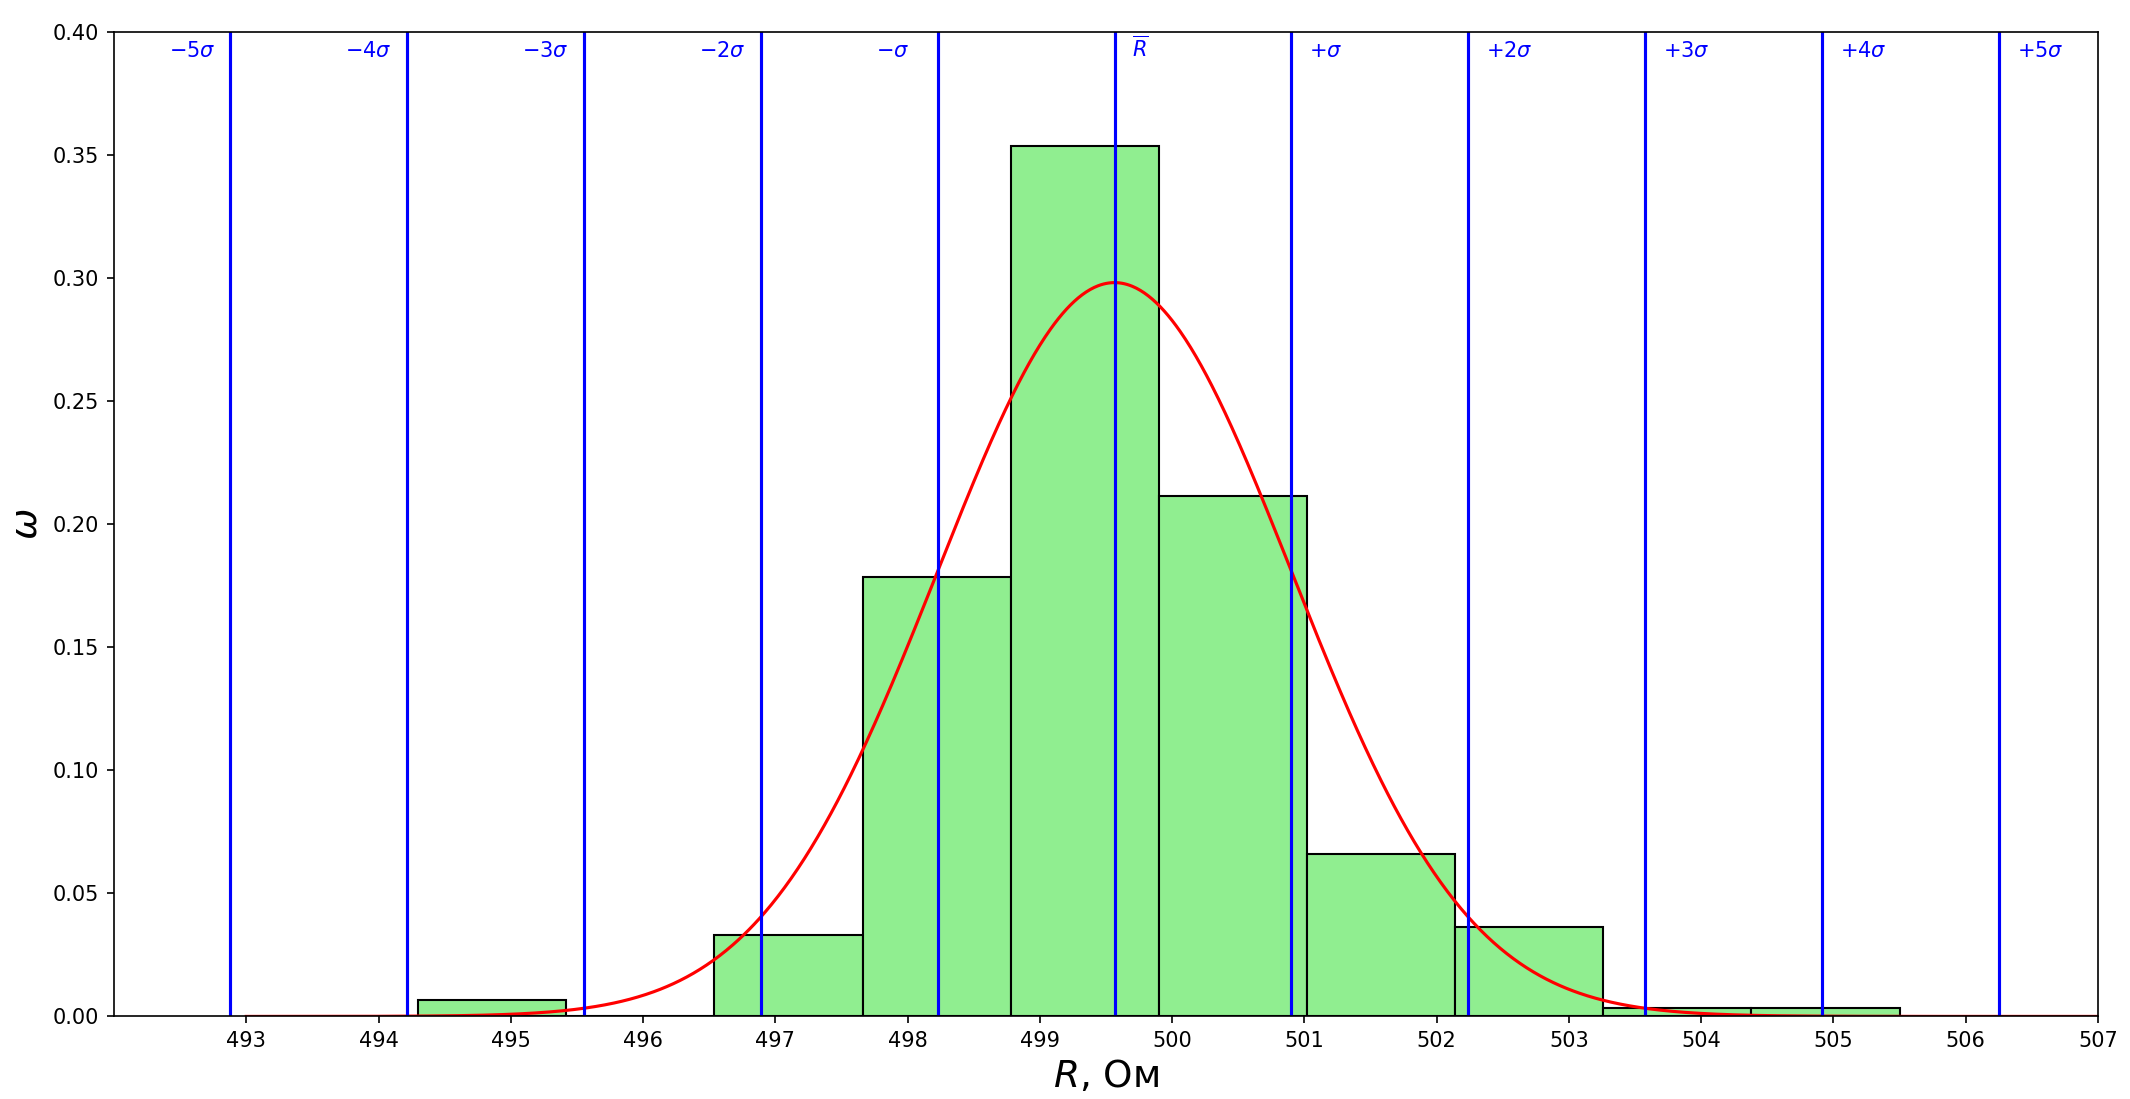
\includegraphics[scale=0.5]{hist1.png}
\end{figure}

\begin{figure}[h!]
\centering
\label{hist2}
\caption{Гисторамма ($m=$20) и нормальное распределение}
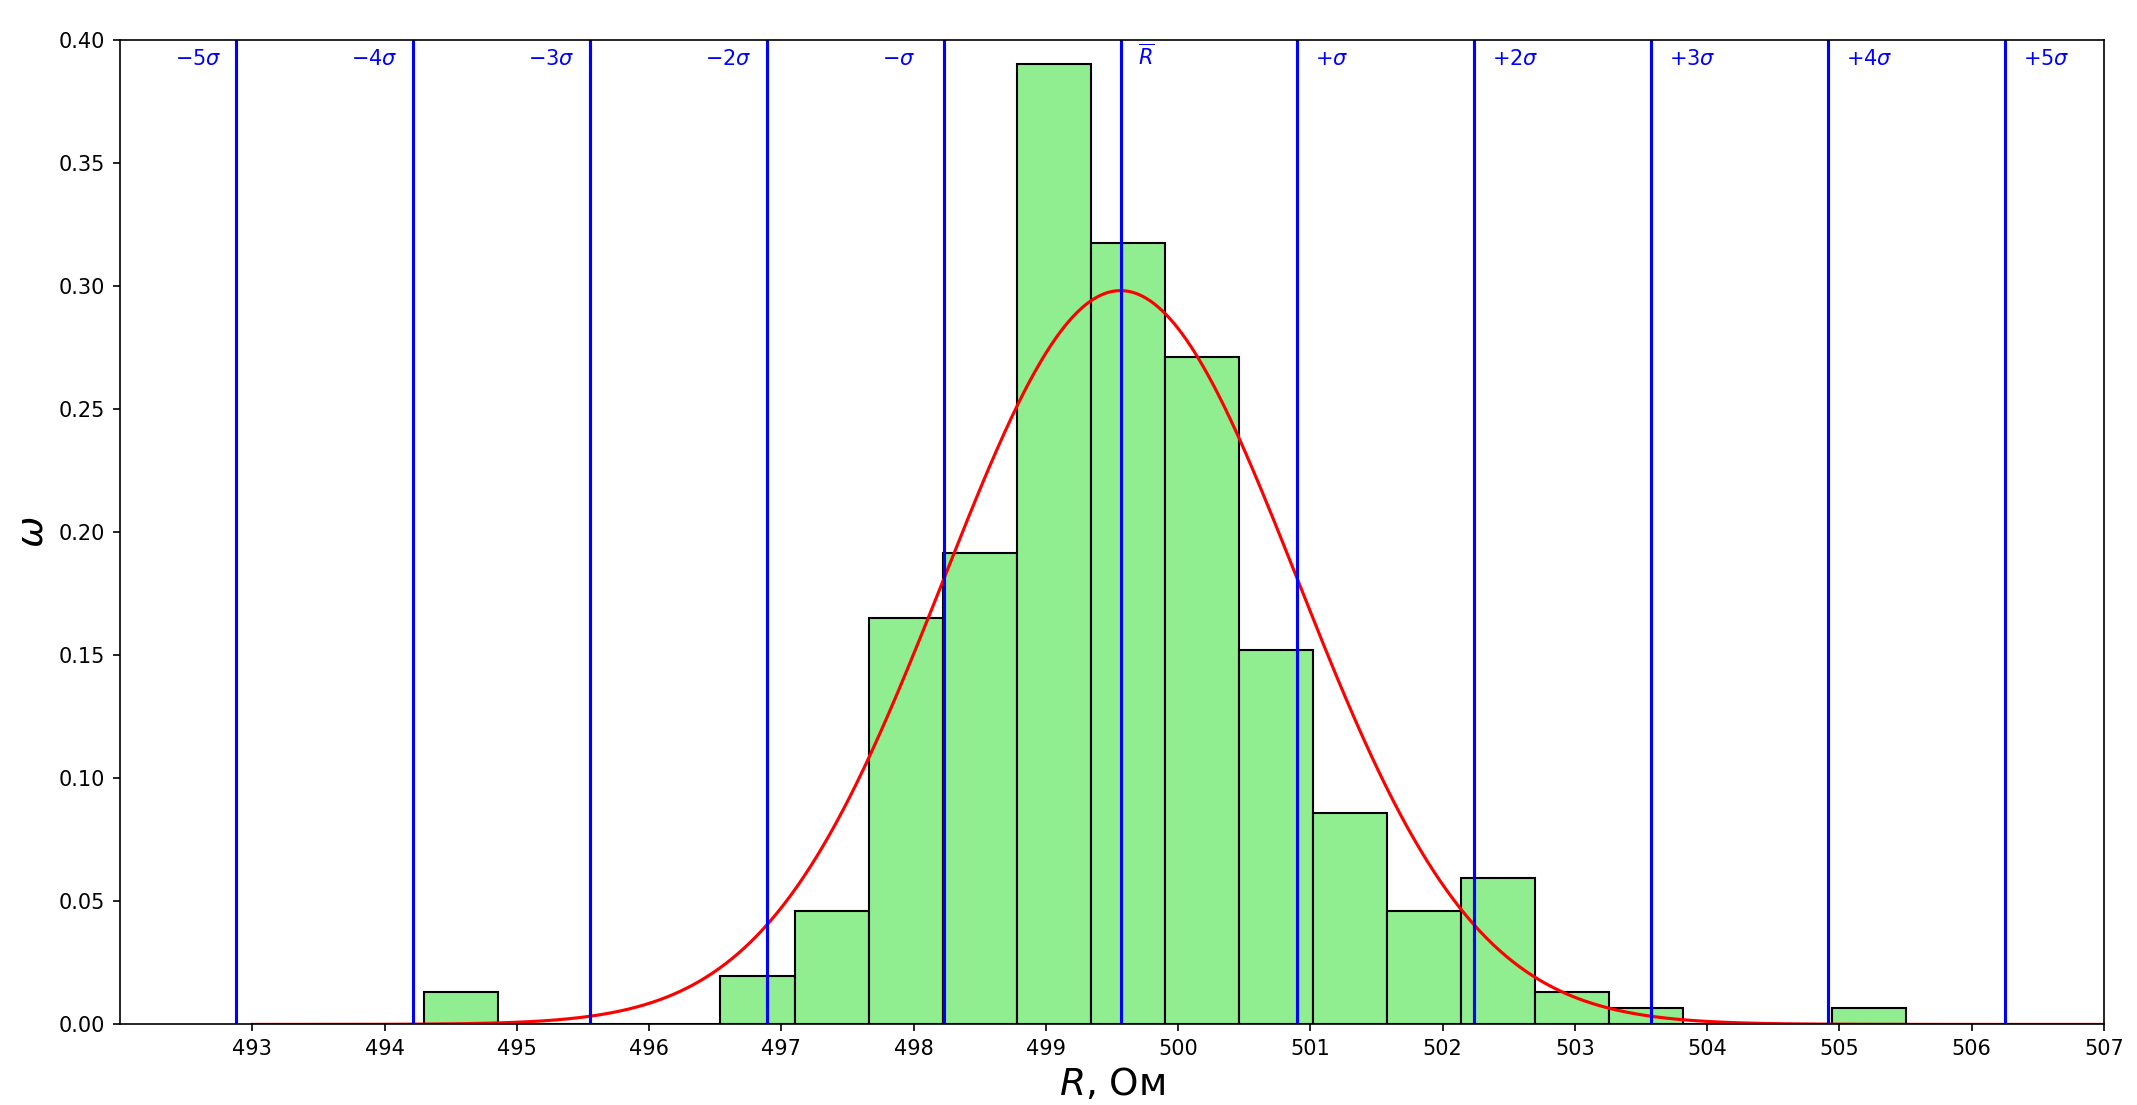
\includegraphics[scale=0.5]{hist2.png}
\end{figure}

\pagebreak
\section{Выводы}
Из рисунков 1 и 2 видно, что гистограммы схожи с кривой нормального распределения, но гистограмма на рисунке 2 ближе, из-за большего количества интервалов измерения.

Ведичина сопротивления резистора, наугад выбранного из данного набора, попадает в интервал $499,56 \pm 1,34$ Ом c вероятностью 72,6 \%, в интервал $499,56 \pm 2,68$ Ом c вероятностью 94,8 \%, в интервал $499,56 \pm 4,02$ Ом c вероятностью 98,5 \%, в интервал $499,56 \pm 5,36$ Ом c вероятностью 99,6 \%, в интервал $499,56 \pm 6,70$ Ом c вероятностью 100 \%

Величины всех сопротивлений из набора укладываются в интервал $499,56 \pm 6,70 (\pm 1,3 \%)$
\end{document}